%%%%%%%%%%%%%%%%%%%%%%%%%%%%%%%%%%%%%%%%%
% Beamer Presentation
% LaTeX Template
% Version 1.0 (10/11/12)
%
% This template has been downloaded from:
% http://www.LaTeXTemplates.com
%
% License:
% CC BY-NC-SA 3.0 (http://creativecommons.org/licenses/by-nc-sa/3.0/)
%

%----------------------------------------------------------------------------------------
%	PACKAGES AND THEMES
%----------------------------------------------------------------------------------------

\documentclass{beamer}

\mode<presentation> {

% The Beamer class comes with a number of default slide themes
% which change the colors and layouts of slides. Below this is a list
% of all the themes, uncomment each in turn to see what they look like.

%\usetheme{default}
%\usetheme{AnnArbor}
%\usetheme{Antibes}
%\usetheme{Bergen}
%\usetheme{Berkeley}
%\usetheme{Berlin}
%\usetheme{Boadilla}
%\usetheme{CambridgeUS}
%\usetheme{Copenhagen}
%\usetheme{Darmstadt}
%\usetheme{Dresden}
%\usetheme{Frankfurt}
%\usetheme{Goettingen}
%\usetheme{Hannover}
%\usetheme{Ilmenau}
%\usetheme{JuanLesPins}
%\usetheme{Luebeck}
\usetheme{Madrid}
%\usetheme{Malmoe}
%\usetheme{Marburg}
%\usetheme{Montpellier}
%\usetheme{PaloAlto}
%\usetheme{Pittsburgh}
%\usetheme{Rochester}
%\usetheme{Singapore}
%\usetheme{Szeged}
%\usetheme{Warsaw}

% As well as themes, the Beamer class has a number of color themes
% for any slide theme. Uncomment each of these in turn to see how it
% changes the colors of your current slide theme.

%\usecolortheme{albatross}
%\usecolortheme{beaver}
%\usecolortheme{beetle}
%\usecolortheme{crane}
%\usecolortheme{dolphin}
%\usecolortheme{dove}
%\usecolortheme{fly}
%\usecolortheme{lily}
%\usecolortheme{orchid}
%\usecolortheme{rose}
%\usecolortheme{seagull}
%\usecolortheme{seahorse}
%\usecolortheme{whale}
%\usecolortheme{wolverine}

%\setbeamertemplate{footline} % To remove the footer line in all slides uncomment this line
%\setbeamertemplate{footline}[page number] % To replace the footer line in all slides with a simple slide count uncomment this line

%\setbeamertemplate{navigation symbols}{} % To remove the navigation symbols from the bottom of all slides uncomment this line
}

\usepackage{graphicx} % Allows including images
\usepackage{booktabs} % Allows the use of \toprule, \midrule and \bottomrule in tables
\usepackage{ulem} %strikethrough effect

%----------------------------------------------------------------------------------------
%	TITLE PAGE
%----------------------------------------------------------------------------------------

\title[undecided]{Not sure yet} % The short title appears at the bottom of every slide, the full title is only on the title page

\author{Michael Carlise} % Your name
\institute[WVU] % Your institution as it will appear on the bottom of every slide, may be shorthand to save space
{
West Virginia University \\ % Your institution for the title page
\medskip
\textit{mcarlise@mail.wvu.edu} % Your email address
}
\date{\today} % Date, can be changed to a custom date

\begin{document}

\begin{frame}
\titlepage % Print the title page as the first slide
\end{frame}

%\begin{frame}
%\frametitle{Overview} % Table of contents slide, comment this block out to remove it
%\tableofcontents % Throughout your presentation, if you choose to use \section{} and \subsection{} commands, these will automatically be printed on this slide as an overview of your presentation
%\end{frame}

%----------------------------------------------------------------------------------------
%	PRESENTATION SLIDES
%----------------------------------------------------------------------------------------



\section{Introduction}

\begin{frame}
		\frametitle{Problem Size/Compute Time Correlation}
			\begin{figure}
					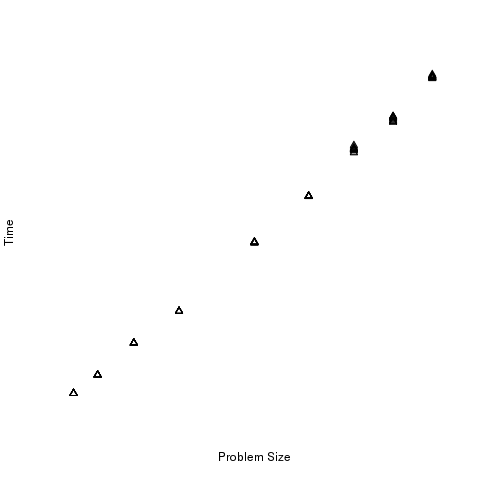
\includegraphics[width=0.65\linewidth]{figures/time/linpack}
			\end{figure}
\end{frame}

\begin{frame}
		\frametitle{Problem Size/Compute Time Correlation}
			\begin{figure}
					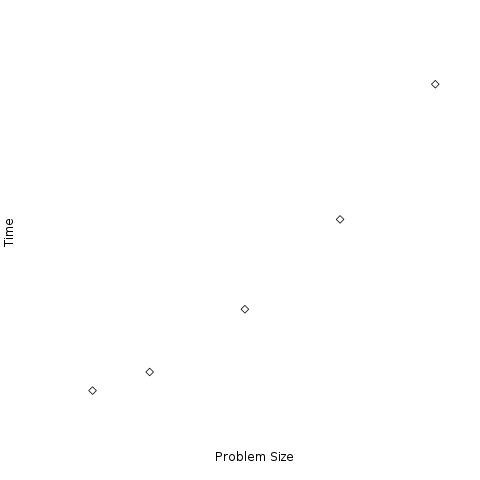
\includegraphics[width=0.65\linewidth]{figures/time/laplace}
			\end{figure}
\end{frame}

\begin{frame}
		\frametitle{Problem Size/Memory Correlation}
			\begin{figure}
					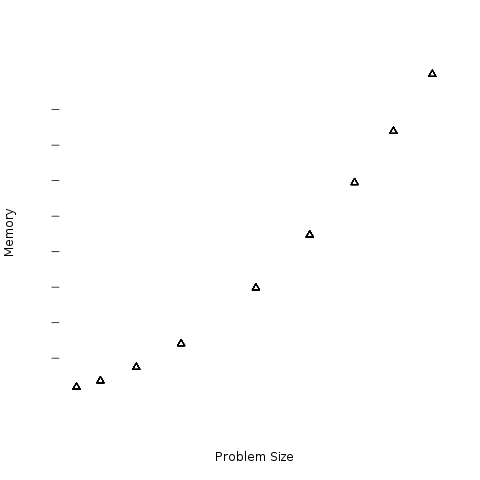
\includegraphics[width=0.65\linewidth]{figures/memory/linpack}
			\end{figure}
\end{frame}

\begin{frame}
		\frametitle{Problem Size/Memory Correlation}
			\begin{figure}
			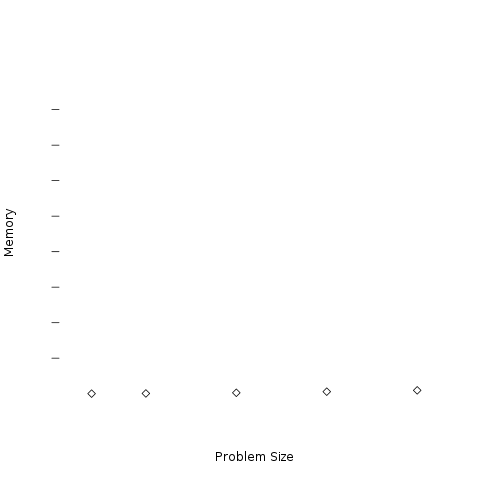
\includegraphics[width=0.65\linewidth]{figures/memory/laplace}
			\end{figure}
\end{frame}

\begin{frame}
		\frametitle{Combinations}
		\begin{itemize}
				\item Compute time increases only
				\item Memory usage increases only
				\item Compute time and Memory increases
		\end{itemize}
\end{frame}



\begin{frame}
		\begin{figure}
				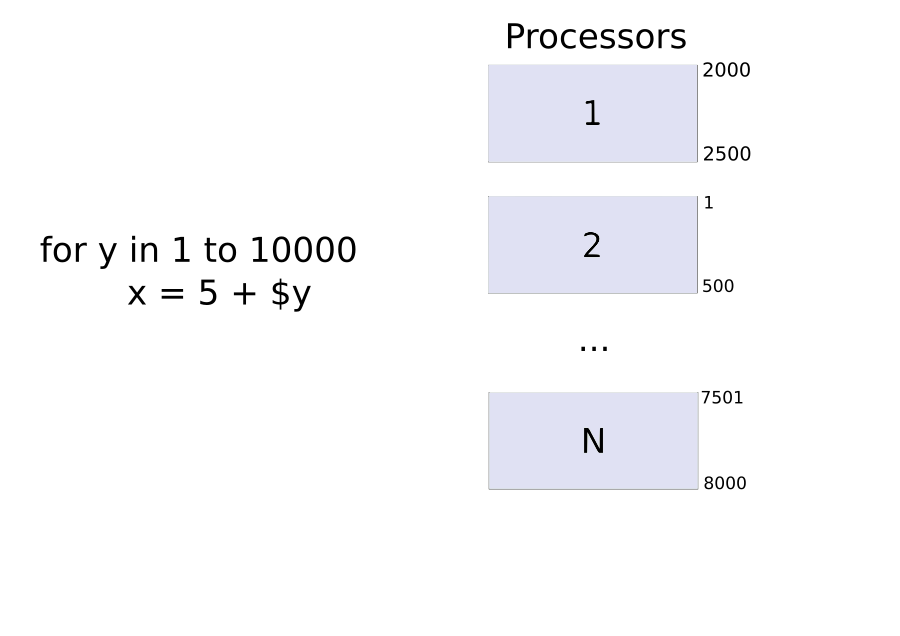
\includegraphics[width=0.8\linewidth]{figures/diagrams/forloop/fordiagram}
		\end{figure}	
\end{frame}

\begin{frame}
		\begin{figure}
				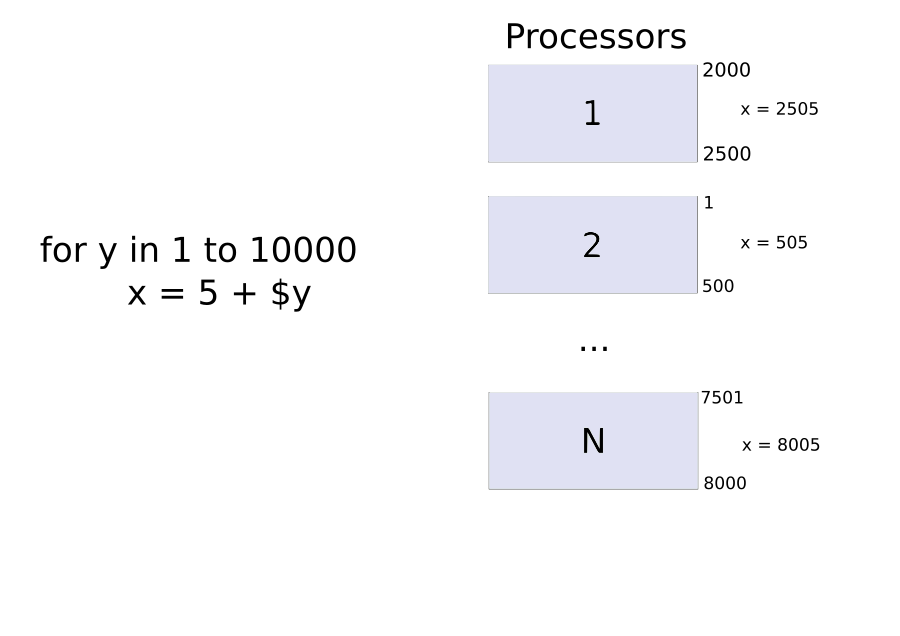
\includegraphics[width=0.8\linewidth]{figures/diagrams/forloop/fordiagram2}
		\end{figure}	
\end{frame}

\begin{frame}
		CLI examples of parallel utilities
\end{frame}


\begin{frame}[fragile]
		\frametitle{R parallel package}
		\center
		\begin{verbatim}
			library(doParallel)
			cl <- makeCluster(2)
			registerDoParallel(cl)
			foreach(i=1:3) %dopar% sqrt(i)
		\end{verbatim}
\end{frame}

\begin{frame}
		observed/expected speedup (figure)
\end{frame}

\begin{frame}
		Amdahl's law (code diagram)
\end{frame}

\begin{frame}
		Parallelization overhead (code diagram)
\end{frame}




\begin{frame}
		\begin{figure}
				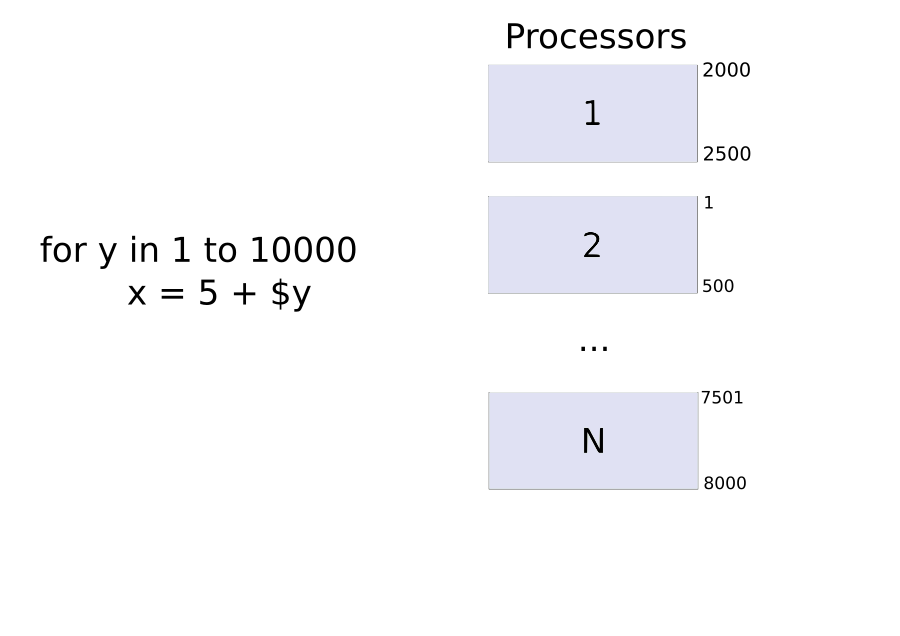
\includegraphics[width=0.8\linewidth]{figures/diagrams/forloop/fordiagram}
		\end{figure}	
\end{frame}

\begin{frame}
		\begin{figure}
				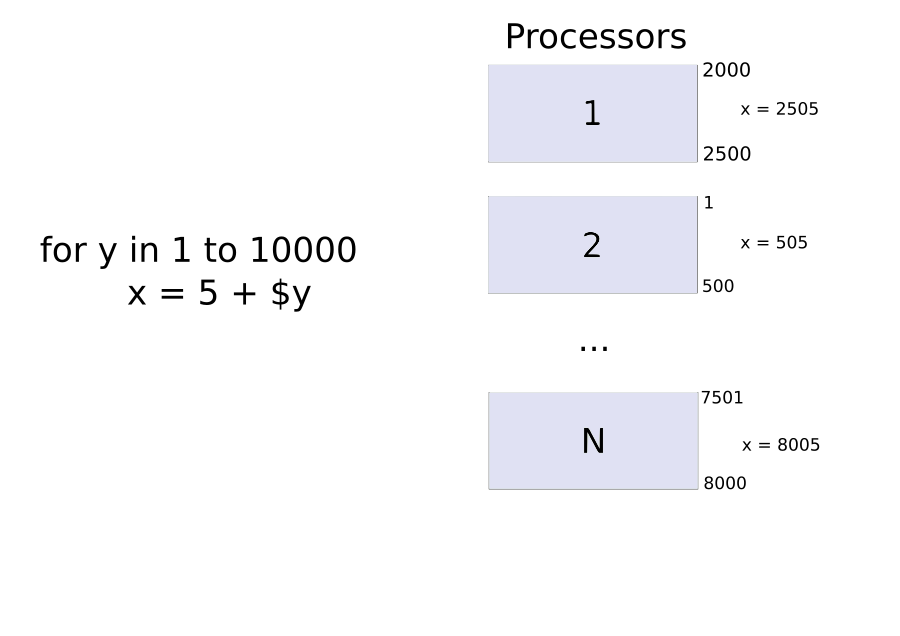
\includegraphics[width=0.8\linewidth]{figures/diagrams/forloop/fordiagram2}
		\end{figure}	
\end{frame}

\begin{frame}
		CLI examples of parallel utilities
\end{frame}


\begin{frame}[fragile]
		\frametitle{R parallel package}
		\center
		\begin{verbatim}
			library(doParallel)
			cl <- makeCluster(2)
			registerDoParallel(cl)
			foreach(i=1:3) %dopar% sqrt(i)
		\end{verbatim}
\end{frame}

\begin{frame}
		observed/expected speedup (figure)
\end{frame}

\begin{frame}
		Amdahl's law (code diagram)
\end{frame}

\begin{frame}
		Parallelization overhead (code diagram)
\end{frame}




\begin{frame}
		\frametitle{Extreme Scientific and Engineering Discovery Environment}
		www.xsede.org
\end{frame}

\begin{frame}
		\frametitle{Online}
		wvuhpc.github.io/bigData
\end{frame}


\end{document} 
